\subsubsection{Settings}
The settings sketch can be seen in \cref{SettingsScreen} and is divided into two sketches. The right sketch shows an expanded list of settings, and the left sketch show the collapsed list of settings.

\begin{figure}[H]
	\centering
    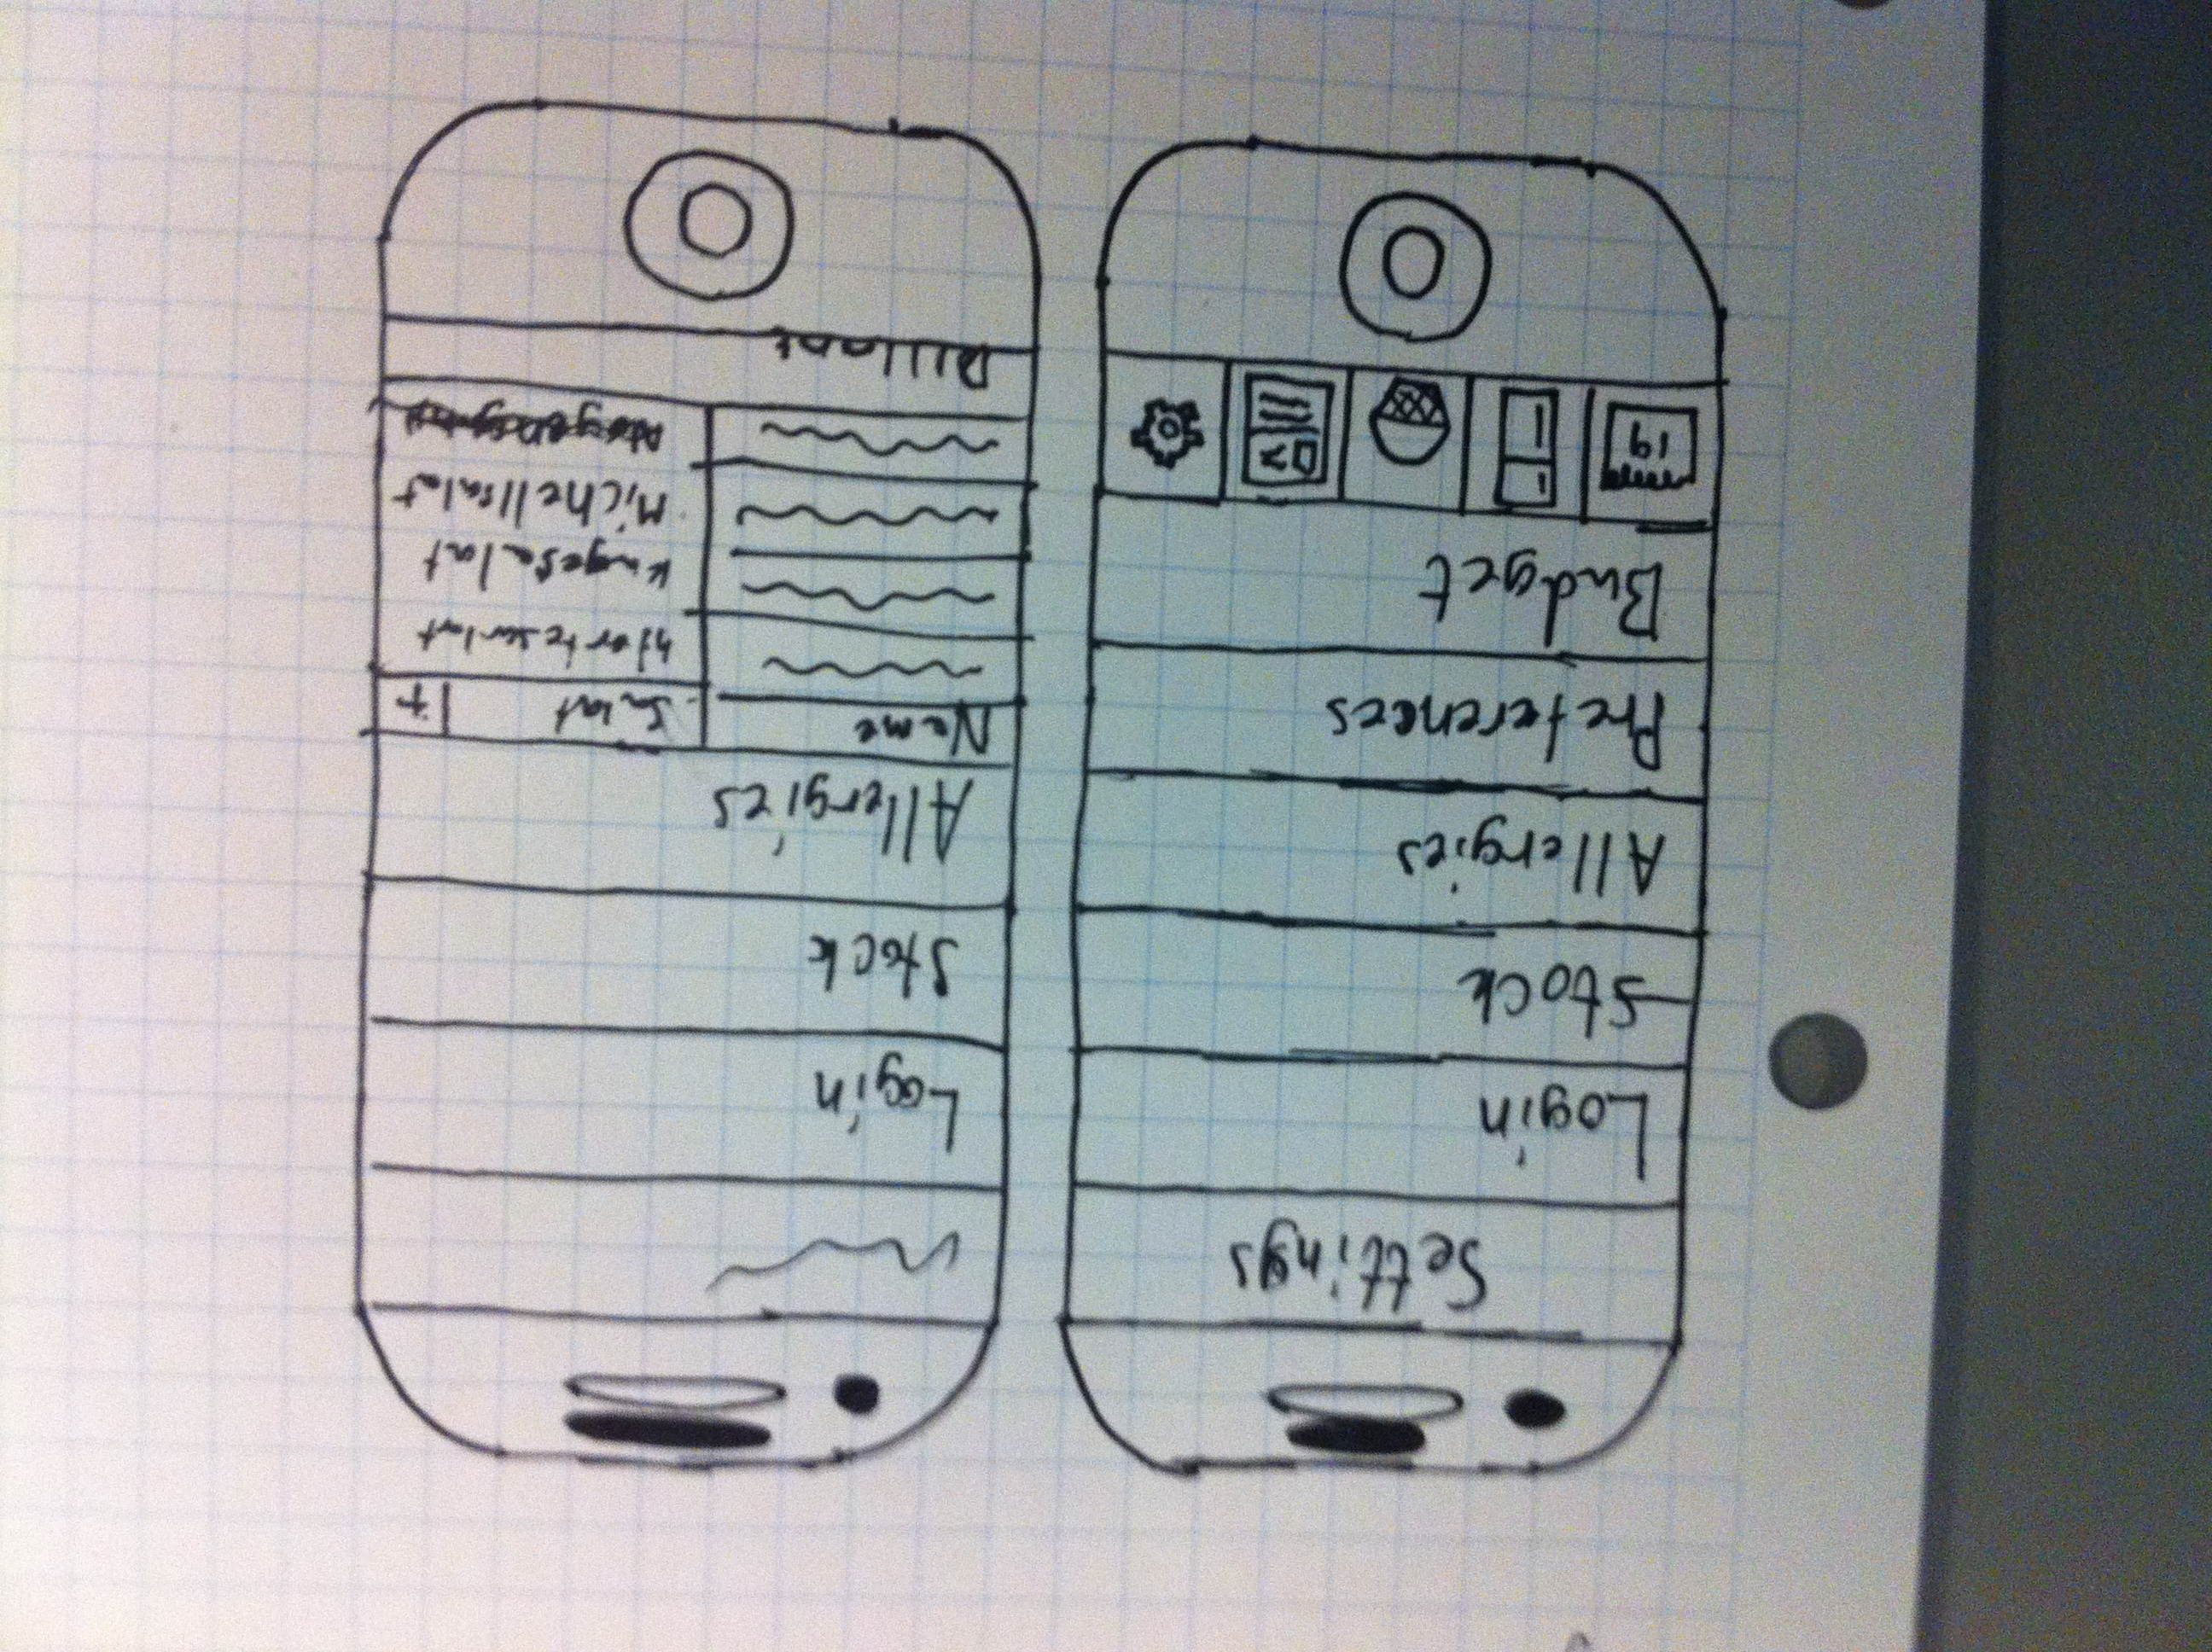
\includegraphics[width=0.5\textwidth]{Grafik/FoodPlanner/FinalSettingsSketch}
	\caption{Sketch displaying all of the settings in the program. With allergies expanded on the right screen.}
	\label{SettingsScreen}
\end{figure}

\textbf{Settings list:}
The settings list is the left sketch in \cref{SettingsScreen} and show a list of settings. The settings can be scrolled through, by swiping up and down, if more settings are needed than the screen can hold. The items shown in the sketch are just ideas for settings, and are just used to visualize the design idea. These are not all settings that will be incorporated in the program.

\textbf{Expanded settings list:}
The right sketch in \cref{SettingsScreen} shows the list of settings, as described in the settings list paragraph above. Furthermore, this sketch has an expanded setting. This is because if a user click a setting, it will expand, and show more information about this setting. In the sketch, allergies is expanded.

Expanding was chosen, because it would be consistent with the rest of the program, instead of other ideas that where discussed, for example a pop up. 